\documentclass[runningheads,a4paper]{llncs}
    
\usepackage[utf8]{inputenc}

\usepackage{varwidth} \usepackage{linegoal} \usepackage{POE}
\usepackage{amssymb} \usepackage{dsfont} \usepackage{stmaryrd}
\usepackage{comment} \usepackage{graphicx}
\usepackage[textsize=tiny,textwidth=\marginparwidth]{todonotes}
\usepackage{url} \newcommand{\keywords}[1]{\par\addvspace\baselineskip
  \noindent\keywordname\enspace\ignorespaces#1}
\usepackage{NewItMathFont}
\renewcommand*{\mprintsingle}[2]{\mathsf{#1}}%
\renewcommand*{\mprintmulti}[2]{\mathit{#1}}%
\usepackage[inline]{enumitem} \usepackage{wrapfig}
\usepackage{collectbox}
\usepackage{natbib}

\makeatletter \newcommand{\mybox}{%
  \collectbox{%
    \setlength{\fboxsep}{1pt}%
    \fbox{\BOXCONTENT}%
  }%
}


\begin{document}

\mainmatter

\title{POE-$\Delta$ Towards a formal framework for change} \titlerunning{Towards a formal framework for change}

\author{Georgi \textsc{Markov} \and Jon G. \textsc{Hall} \and Lucia
  \textsc{Rapanotti}} \authorrunning{Markov, Hall, Rapanotti}


\institute{Department of Computing and Communications\\
  The Open University, UK\\
  \url{{georgi.markov, jon.hall, lucia.rapanotti}@open.ac.uk} }

\toctitle{POE-$\Delta$ Towards a formal framework for change} \tocauthor{Markov, Hall, Rapanotti}
\maketitle


\begin{abstract}
  TBD \keywords{TBD}
\end{abstract}

\section{Introduction}
\label{sect:Intro}

Change has received little interest from formal methods\todo{Check}. 

%
%
%Hybrid systems refer to systems exhibiting a mix of discrete and
%continuous behaviour - continuous change of the system state as well
%as discrete transition of states
%\citep{prabhakar2016counterexample}. As such they present an
%appropriate paradigm for modelling (real-time) embedded control
%systems \citet{papp2015embedded} which represent the driving force for
%technological development in many modern domains, including but not
%limited to automotive, healthcare, industrial automation, and so on
%\cite{anand2010generating}. This makes hybrid system theories profound
%for the analysis and reasoning in these important and difficult
%domains.
%
%While there are several different such theories, they all consist of
%some combination of differential equations and automata for capturing
%the dynamic and discrete part of the systems behaviour. From a system
%architect's perspective, however, this represents only one of several
%important viewpoints necessary for the design of a software-intense
%system (for example see the 4+1 architectural view model
%\cite{Wikipedia:2016aa}), and Hybrid System theories are clearly
%lacking a way to express system structure. Additionally, the
%mathematical basis of most such theories does not lend itself well to
%the majority of practitioners which hampers the creation of a
%adequate, complete, and consistent multi-view model of the to be
%designed system.
%
%In this paper, we try to take steps towards closing this gap by
%reinterpreting one of the more popular hybrid system theories -
%Chaochen's Hybrid CSP (HCSP)\cite{chaochen1996formal}, based on
%Hoare's CPS \cite{hoare1985communicating}, in terms of real-world
%phenomena - the units of both - behaviour and structure, and then
%integrate this, now phenomena-based, HCSP in our design theories for
%greenfield and brownfield problems \POE{} (POE), and POE-$\Delta$
%\todo{citation - Journal}. The paper does not attempt to be exhaustive
%in our coverage of topics; but we will provide references for further
%study.
  
The remainder of this paper is organised as follows: \todo{Paper
  layout}

\section{Background}
\label{sect:background}

%\subsection{A Calculus for Hybrid CSP}
%\label{subsect:intr.calc4hcsp}
%Chaochen's Hybrid CSP \cite{chaochen1996formal} extends Hoare's
%original CSP language \cite{hoare1985communicating} with continuous
%variables, differential equations, time and other constructs necessary
%to model the different aspects (i.e. continuous, communicating,
%real-time, etc.) of the behaviour of hybrid systems. The final
%vocabulary of the HSCP language includes three sets of disjoint
%alphabets: a set of discrete variable - $Var$, a set of continuous
%variables expressed as functions of time - $State$ and a set of
%channels $Chan$ (which can be further subdivided in InChan - for input
%channels, and OutChan - for output channels) to facilitate the
%communication between processes \cite{Liu2010}. The following
%represents a summary of the HSCP grammar in BNF (similar summaries can
%be also found in \cite{chaochen1996formal}, \cite{Liu2010} and
%\cite{guelev2013super}:
%
%\[\footnotesize\begin{array}{rcll}
%                 SP &:=& P \mid S \mid P \parallel S \\ 
%                 P &:=& stop \mid skip \mid v := e \mid ch?x \mid ch!e \mid \rightarrow P_{i}) \mid \langle F(\dot{s} ,s) = 0 \rangle \mid \langle F(\dot{s} ,s) = 0 \rangle_{e} \\
%                 S &:=& P;Q \mid P \rightarrow B \mid B \rightarrow P \mid P \trianglerighteq_{d} Q \mid P \trianglerighteq_{d} []_{i \in I}(io_{i} \rightarrow Q_{i}) \mid \mu X . F(X)
%	
%               \end{array}\]
%             where
%             \begin{itemize}
%             \item $s$ and $\dot{s}$ represent vectors of variables,
%               respectively their derivatives over time.
%             \item $ch$ is a channel name.
%             \item $I$ represents a set of indices.
%             \item $e$ and $B$ are arithmetic and boolean expressions,
%               respectively.
%             \item $d$ is a positive real constant.
%             \item $stop$ does nothing and just keeps idle forever.
%             \item $skip$ does nothing and terminates immediately.
%             \item $v := e$ assigns the value of the expression e to
%               v, then terminates.
%             \item $ch?x$ receives a value to x on channel ch.
%             \item $ch!e$ sends the value of the expression e on the
%               channel ch.
%             \item $\langle F(\dot{s} ,s) = 0 \rangle$ is a
%               differential equation representing an evolution by
%               means of a differential equation over s.
%             \item $\langle F(\dot{s} ,s) = 0 \rangle_{e}$ is another
%               differential equation which behaves as the one above
%               but resets the value of s to e.
%             \item P; Q behaves like P at first, and once P
%               terminates, it behaves like Q.
%             \item $P \rightarrow B$ behaves like P until B becomes
%               true, then it terminates.
%             \item $B \rightarrow P$ behaves like P if B is true, else
%               it terminates.
%             \item $P \trianglerighteq_{d} Q$ behaves like P if P can
%               terminate within d seconds. If not it behaves like P
%               initially and after d seconds switches the behaviour to
%               Q.
%             \item
%               $P \trianglerighteq_{d} []_{i \in I}(io_{i} \rightarrow
%               Q_{i})$ Behaves like P if P can terminate within d
%               seconds. If not it behaves like P until a communication
%               (io - input or output) appears, after which it switches
%               to $Q_{i}$.
%             \item $\mu X . F(X)$ describes a tail-recursive process
%             \item $P \parallel Q$ behaves like if P and Q are
%               executed independently with the only exception that all
%               communications along a shared channel have to be
%               synchronised.
%             \end{itemize}
%
%             In the following we demonstrate the use of HCSP to
%             specify and reason about properties of the behaviour of a
%             hybrid system on a very simple example, which we will
%             reuse thorough the paper to illustrate different concepts
%             from in the context of our idea. The example considers
%             the Inventory Management System (IMS), introduced in
%             \cite{chaochen1996formal}, whose behaviour can be
%             described as follows in HCSP:
%
%$$ ch?x; (\langle (\dot{x}) = -\alpha + \beta \rangle) \triangleright ch?\beta $$
%and where:
%\begin{itemize}
%\item $x$ represents the IMS' stock.
%\item $\alpha$ represents the utilisation dynamic.
%\item $\beta$ represents the amount of a new order.
%\item $(\dot{x}) = -\alpha + \beta$ represents the IMS' behaviour
%  after it receives a new order of amount $\beta$.
%\end{itemize}
%
%While such a system description is useful for reasoning about the
%dynamics of the system, it is also incomplete and insufficient for a
%successful system synthesis, as it omits any explicit information from
%a logical or physical views of the system could be derived. This is
%what our contribution will try to address. \todo{Expand on the example
%  and the conclusion}

\subsection{POE \& POE-$\Delta$, and the notion of Phenomena}
\label{subsect:intr.poe}
\POE{}, defined by the second and third authors, is an engineering
framework with an accumulated body of work spanning over a decade,
including application and evaluation through a number of real-world
engineering case studies. Its underlying design theory concerns the
characterisation of individual problems and how problems relate and
transform to other problems as part of problem solving processes.

\POE{}-$\Delta$ is a recent extension to POE which shares and expands
on a number of \POE{}'s characteristics, including elements of its
semantics; its graphical notations; and its underlying process pattern
\cite{Hall2009JAdvSysMeas}. However, while \POE{} deals with
`greenfield' development, \POE{}-$\Delta$ deal with change, or
`brownfield,' problems which are solved not solely by the design of a
new artefact, but by a change of, and addition to, existing artefacts
within a target context (a system, product, process, etc).

A thorough presentation of POE and POE-$\Delta$ is beyond the scope of
this paper, but can be found in \cite{hall2016a-design}, respectively
\todo{add reference to POE-$\Delta$}. Here, we very briefly recall
some basic definitions and concepts important in the context of this
paper.

In POE a problem is ``a stakeholder's recognised need in context.''
For stakeholder $G$, with recognised need $N_G$ in real world context
$E_G$, we defined their problem to be the pair:
%
\[(E_G,N_G)\]
%

$E_G$ and $N_G$ are to be understood only as place holders, as $G$'s
initial conceptualisation of their problem may have neither solution
nor sense. Irrespective of sense or solution existence, $G$'s wish
becomes a challenge to designer $D$ to make sense of $G$'s problem by
finding an agreed environment $E$ and need $N$, leading to $D$'s
problem
%
\[E(S)\meets_{G}N\]
%
which reads ``Find $S$ which, when installed in $E$, meets $N$ to the
satisfaction of $G$.''

$D$'s challenge consists of all the solving problems activities that
lead to the solution of $G$'s problem. Someway through problem solving
we encounter $D$'s variously detailed $E$, $N$ and $S$ and form a
judgement as to whether a problem has been solved. We do this by
creating a solution for it through a sequence of judgement-preserving
transformations, i.e., transformations that the relevant stakeholders
would agree preserved solvability, that move a problem to known solved
problems. Thus, a problem is solved if and only if it can be
transformed to known solved problems. As part of the transformation
sequence, a solution to the problem is created.

In POE-$\Delta$, we begin from the same place as \POE{}: we suppose
that change problem owner $G$ recognises a need in the real world and
wishes that need to be satisfied. From $G$'s perspective, then, a
problem $P$ is a pair, consisting of a real world context $E_G$ and a
need $N_G$.


Irrespective of sense or solution existence, we will assume that $G$'s
wish becomes a challenge to a change engineer $D$ to make sense of
$G$'s change problem $(E_G,N_G)$ and to solve it. $D$'s challenge thus
consists of (cf. \cite{hall2016a-design}):
%
\begin{enumerate}[label=CPS\arabic*.]
  % \begin{enumerate}
\item creating their own view, $(E, N)$, of the $G$'s change problem
  $(E_G, N_G)$, and identifying domains that must remain unchanged, those that can change;
\item receiving validation from $G$ that $(E, N)$ is properly
  representative;
\item either, identifying a new environment $F$ satisfying the change need which 
\begin{enumerate}[label=\roman*.]
\item preserves those  parts of $E$ that should remain unchanged, 
\item identifies any changes necessary to domains that can change, and 
\item identifies any additional domains necessary to effect the change;
\end{enumerate}
or reporting that the change isn't possible.
\item receiving validation from $G$ that $F$ meets the agreed
  recognised changed need $N$;
\item migrating from $E$ to $F$.
\end{enumerate}

Like \POE{} \cite{hall2016a-design}, even if expressed linearly as
bullet points, the challenge facing $D$ may be iterative and highly
non-linear.

Although $E_G$ and $N_G$ are expressed in stakeholder language, here we assume that the developer has access to a full formal tool box and is able to express both $E$ and $N$ in a suitable formal language. For this paper, we assume that language is Hybrid CSP \cite{chaochen1996formal}.

\subsection{Running example: a kettle}

\begin{figure}[hbt]
\centering{
  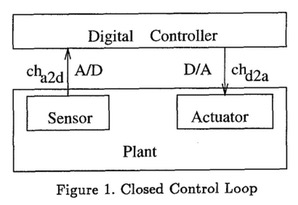
\includegraphics[width=0.6\textwidth]{img/iPlant}}
  \caption{The Interfaced Plant problem \cite{chaochen1996formal}}
  \label{fig:iPlant}
\end{figure}
\begin{example}

\todo{this}Introduce example of a kettle, as in OmniGraffle file. This is actually a quite general Plant/Controller situation and so lessons from this example extend quite far.

%
\end{example}

The intention is to change the algorithm, $ALG$, which controls the kettle.

\subsection{CPS1: Hybrid CSP}

\todo{move intro to HCSP here. Add the modelling of phenomena; description of $E[S]\models N$ in HCSP}

Kettle is: (adapted from \cite{chaochen1996formal} InterfacedPlant example)

\[Kettle :: \left\langle 
\begin{array}{rcl}
 y&=&temp(x)\\
 \dot{x}&=&f(x,u)\\
 \dot{u}&=&0\\
\end{array}\right\rangle
\]
%
where $f(x,on) = 1^\circ C/sec$ and $f(x,off) = 0^\circ C/sec$.

\[Program :: (u := on\triangleright_T (ch_{a2d}?y; u := ALG(y,u); ch_{d2a}!u) )\]
where 
%
\[ALG(y,u) = if \ y > 90^\circ C \ then \ u = off \ else \ u = on \ fi\]
%
and
%
\[InterfacedKettle :: (Kettle \triangleright (ch_{a2d}!y ; ch_{d2a}?u) )\]

Composed system is 
\[InterfacedKettle[Program]\]

\todo{Should be expressed in terms of a figure (OmniGraffle) that corresponds to the formal description in terms of HCSP semantics, extended to include $E[S]\models N$.}

What is the need? I'd like to be able to [$KNeed$] change the algorithm without compromising safe and live operation of the kettle. So the change problem is:
%
\[InterfacedKettle[Program]\Delta F\models KNeed\]
%
and our task to to find $F$.\todo{What does safe and live operation look like for the kettle?}

To find $F$ we need to identify which domains should remain the same and which can change. This means the new OmniGraffle diagram with possible changes indicated.

\subsection{CPS2: Validating a formal description}

\todo{something on validation of formal expressions here, show your implementation in python; work on implementation. Needs scholarship on literature.}

\subsection{CPS3: describing the change}

\newcommand{\replacedBy}{\triangleright}

Given the above, we consider a formal change problem to be a four-tuple, written $E\Delta F\meets_G N$ where $E$ and $F$ are both collections of domains (although $F$ can have abbreviated expression, see later) and $N$ is a description of a change need. Unlike $E$ which is arrived at from an understanding of the real world, $F$ is a designed object, validated in CPS4.

\todo{Then something leading into this} 

As such, and without constraining the languages in which existing and new components are or will be expressed, it is constrained in the forms it can take by the following grammar:
%
\[\footnotesize\begin{array}{rcll}
                 ChangeDomain &:=& Domain \mid Domain[\{Changeable\}](\{NewDomain\})\\
                 Changeable &:=& ChangeDomain \mid CP \mid \cancel{Domain} \mid Domain \replacedBy NewDomain\\
                 Domain, NewDomain, Need &:=& Name
               \end{array}\]
               
\subsection{CPS4: validating the change}

Again, this might include some animation of the entire system so that.

\subsection{CPS5: making the change}

This determines the structural constraints on the change. However. change also affects behaviours. Which mechanisms do we have that allow us to reason about behavioural changes.

Because of the semantics of parallel as constraining conjunction, a component removed will relax constraints, increasing possible behaviours. A subsequently replaced component will again restrict the behaviours. The process of decommissioning the old system and commissioning the new is then visiting the unconstrained behaviour followed by the newly reconstrained.

Given a fmdl term $e$, in which a subsystem $f$ has been identified through the above grammar, so that $e = e[f]$, say, the decommissioning of $f$ is modelled by $e = e[f]$ to $e[chaos]$. Commissioning of the new component $f'$ is then $e[f']$.

Thus we have the relationships:
%
\[e[f]\subseteq e[chaos]\supseteq e[f']\]
%
and managed chain means that exists $I$ such that:
%
\[I\models (e[f]^\frown e[chaos]^\frown e[f'])\land N\]

*****

             From the grammar above we can see that Domains represent
             a crucial concept in POE and POE-$\Delta$. Domains,
             however, are simply a named collections of phenomena:
             events, entities, values, etc., connected by shared
             phenomena. In POE and POE-$\Delta$, the different aspects
             of a problem's description, i.e. the problem's
             environment $E$, are represented through sets of
             \textit{domains}, each a set of related
             \textit{phenomena} that are usefully treated as a unit
             for the purpose of problem solving (c.f., \cite[Page
             270]{Jackson2001}). In general, treatment of the physical
             world in POE and POE-$\Delta$ is based on the work of
             Jackson and others
             \cite{896248,Jackson2001,hall2003reference}, which relies
             on the notion of real-world phenomena and their
             relationships. For the purpose of this discussion, a
             phenomenon can be simply characterised as ``an element of
             what we can observe in the world.'' This definition
             suggests both structural and behavioural characteristics
             \cite{hall2003reference}:
             \begin{itemize}
             \item As a structure, an environment $E$ is a collection
               of domains $[D_{1},...,D_{n}]$, suggesting that in
               POE/POE-$\Delta$ entities are composed of other
               entities and are related to each other.
             \item behaviourally, a domain maps a collection of
               phenomena to a timeline of their occurrences and
               interactions.
             \end{itemize}

             Thus our goal is to leverage this important
             characteristic of phenomena in trying to reinterpret HCSP
             through them towards creating a common core for both
             calculi and a semantic bridge / mapping between the HCSP
             and POE/POE-$\Delta$ domains. In such a way, HCSP will
             gain an additional view, allowing it to complement the
             behavioural description of a hybrid system with a
             structural one. POE and POE-$\Delta$ will gain a
             formalism, which will allow its users to gain more
             accuracy using a lower-level (executable) notation.
             
\subsection{The nature of change problems}

CPS3 sketches the relationship between $E$ and $F$. Of course, the most direct --- if not necessarily the most cost-effective --- approach to a change problem is to see it as a greenfield problem ignoring what went before. However, in resource constrained situations, we may wish to preserve some of what already exists, changing only parts. In other situations, it may be necessary to preserve certain subsystems, legacy systems for instance, in the redeveloped system. In general, we would like to change as little as possible and still achieve the change. 

Moreover, the problem owner might wish to specify which parts of the current situation should be preserved going forward. This is problematic, however, as their perception of what should remain changed may not lead us to a solvable problem --- there may be no solution based while those part remain.

To understand the options that this leaves us with, we must look more formally at change problems. Starting form a solved problem, we have three options for change:
%
\begin{itemize}
\item Option i: the environment $E$ of the problem changes, but the need $N$ stays the same. This occurs when, for instance, the environment of the system is volatile \cite{};
\item Option ii: the need $N$ changes, but the environment $E$ stays the same. This occurs when, for instance, the customer's needs change during development;
\item Option iii: both environment $E$ and need $N$ change for a combination of the above reasons;
\item Option iv: the solution $S$ is changed but both $E$ and $N$ are preserved. This might occur when, for instance, we wish to move to a more efficient solution.
\end{itemize}
%
the relationship between these options is shown in the following diagram:
%

\begin{figure}
\[\footnotesize\begin{array}{ccccc}
	&&\textrm{iv. }E[S]\models_G N\rightarrow E[S']\models_G N&&\\
	&\slash && \backslash&\\
\textrm{i. }E'[S]\not\models_G N\rightarrow E'[S']\models_G N&&&&\textrm{iii. }E[S]\not\models_G N'\rightarrow E[S']\models_G N'\\
	&\backslash && \slash&\\
&&\textrm{ii. }E'[S]\not\models_G N'\rightarrow E'[S']\models_G N'&&\\
\end{array}\]
\caption{The four change options that arise.}
\end{figure}



Further to this, a problem owner may wish to specify which elements of a current solution should remain the same, so that we must identify elements of $S$ that should be preserved across change. As the following example shows, this is not always possible.

\todo{Example of Warehouse management system in which environment changes the channel upon which it communicates, but the problem owner refuses to allow the channel on which the solution communicates to change.}

\todo{We need to illustrate each change-type formally. This will give us a formal handle to be able to reason about what can and what can't be done in the various situations.}

Questions:
%
\begin{itemize}
\item can we use Chaochen Section 4.3 --- the Closed Control Loop example --- to illustrate these situations? It's a complex formal example, and there's a lot of room for change.
\item what can we say about the $E'N'$ situation in terms of $E'$ and $N'$ situations?
\item are $E'$ and $N'$ situations fundamentally different, or can they be handled together? 
\item what can we say about behaviours through `probes'?
\item in the first case, we need that $S'$ `implements' $S$, this is probably already a known relationship from formal refinement (Carroll's work at Oxford);
\item 
\end{itemize}



             \section{Towards A Phenomena Based HCSP}
             \label{subsect:phenomhcsp}
             This section discusses central ideas rather than a
             comprehensive presentation of how HSCP and POE/POE-$\Delta$
             can be integrated and how this allows us to capture
             POE/POE-$\Delta$ steps or entire processes in terms of
             HSCP operations and in such a way gives our problem
             calculus a more formal base with executable
             semantics. This is achieved through reinterpretation of
             Chaochen's Hybrid CSP (HCSP) \cite{chaochen1996formal} in
             terms of real-world phenomena and domains which are the
             building blocks of POE/POE-$\Delta$. This allows the
             definition of a semantic function over the two
             description systems, which semi-automatically maps
             between HCSP and POE/POE-$\Delta$.

             \subsection{Unit Domains}
             \label{subsect:phenomhcsp.singlePhenDom}
             Phenomena, as discussed in section
             \ref{subsect:intr.poe}, are the core building blocks of
             both POE and POE-$\Delta$. All higher level constructs% -
             % problems, relationships, context,
             in POE/POE-$\Delta$ are composed of phenomena. In
             \cite{hall2003reference}, phenomena are defined as ``the
             indivisible unit of both behaviour and structure of
             everything we can observe in the world''. As such, all
             HCSP primitive constructs%: (i) the channel, which controls the
             % broadcast of values; (ii) the discrete variable, which
             % holds a constant scalar value, and (iii) the continuous
             % variable, which holds a continuously variable value can
             can be reinterpreted in terms of phenomena. This would
             give us a phenomenological basis for HCSP.

             For this we build upon the notion of POE/POE-$\Delta$
             unit domains which represent domains controlling a single
             phenomena and define the idea of HCSP-domains. A HCSP
             domain is the POE/POE-$\Delta$ representation of a HCSP
             primitive term whose description is the HCSP term itself.

             \begin{figure}[hbt]
               \centering{
                 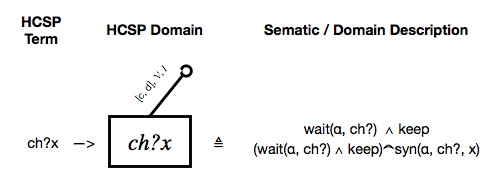
\includegraphics[width=0.9\columnwidth]{img/HCSPDomain}}
               \caption{Representation of HCSP Domain}
               \label{fig:HCSPDomain}
             \end{figure}

             The arc connected to the domain box and it's annotation
             is used for capturing information about shared state,
             including the satisfiability of the term expressed as a
             truth value of the function represented by the respective
             term for the specified interva, and determined by the
             term's value assignments, state and variable
             interpretations in the context of the function's interval
             and finally, l. Therefore it is crucial for the
             representation of more complex HCSP terms in
             POE/POE-$\Delta$ diagrams.
             
             In the following we show how we use this notion of the
             HCSP domain to gain operational semantics of HCSP as part
             of a higher level POE/POE-$\Delta$ calculus.

             \subsection{Semantics of HCSP}
             \label{subsect:phenomhcsp.semantics}
             As a running example we are using the following HCSP
             expression, which combines different HCSP
             primitives (input, output, assignment) and a couple of
             composite operators - i.e (sequential and parallel
             process execution) into a more complex expression:

             \[ch!5 || (ch?x; y := x)\]

             We break the expression into its constituent HCSP simple
             terms:
             \begin{itemize}
             \item Channel Output: $ch!5$
             \item Channel Input: $ch?x$
             \item Value assignment: $y:=x$
             \end{itemize}
             Each such HCSP term's semantic is briefly discussed in the
             following and it is shown how such HCSP simple terms can be
             represented with a single phenomena POE/POE-$\Delta$
             domain.
             
\paragraph{The channel output: ch!5}

In \cite{chaochen1996formal}, the semantics of $ch!5$ are
defined as:
\[\footnotesize\begin{array}{rcll}
                 \llbracket ch!x \rrbracket C \triangleq && wait(\alpha, ch!) \wedge keep \\
                                                         &&\vee \\
                                                         && (wait(\alpha, ch!) \wedge keep) \frown syn(\alpha, ch!, x) \frown C
               \end{array}\]

The following two diagrams \ref{fig:ChannelOutput} provide a visual
representation of these semantics: 

\begin{figure}[hbt]
  \centering{
    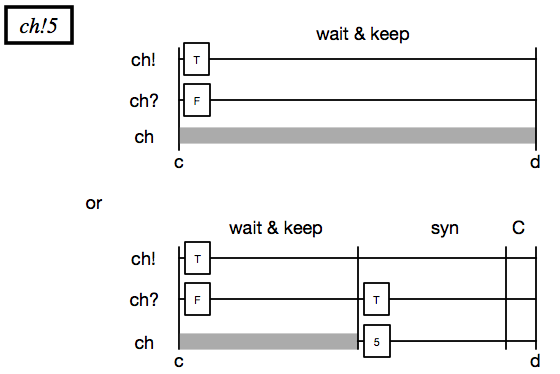
\includegraphics[width=0.9\columnwidth]{img/ChannelOutput}}
  \caption{Graphical depiction of the HCSP channel output semantics}
  \label{fig:ChannelOutput}
\end{figure}

Each diagram presents one of the two cases which satisfy the $ch!5$
semantics. The top diagram depicts the case where $ch!$ it is willing to
communicate (returns $true$ - tt.), while the $ch?$ term returns
$false$- ff., meaning it is unwilling to communicate. In this case the behaviour of $ch!5$ is
characterised by $wait \wedge keep$ and the value on the channel $ch$
is irrelevant.

The bottom diagram, shows the second case, which satisfies the $ch!5$
semantics. It subdivides the $[c, d]$ interval in 3 phases:
\begin{itemize}
\item The first interval segment is analogous to the first diagram -
  $wait \wedge keep$. In the second segment, the value
  of $ch?$ turns to true - tt., meaning that now both - $ch!$
  and $ch?$ are willing to communicate, so we move to the $syn$-phase,
  where the value on the channel $ch$ is send to $x$.
\item The last phase of the interval describes the continuation
  sequence - $C$.
\end{itemize}

The POE/POE-$\Delta$ representation of the ch!5 term is the
\mybox{ch!5} HCSP domain with the following semantic: $\llbracket
ch!5\rrbracket \lceil \rceil$.

\paragraph{The channel input: ch?x}
The next diagram pair \ref{fig:ChannelInput} depicts the second term
in our example - $ch?x$:

\begin{figure}[hbt]
  \centering{
    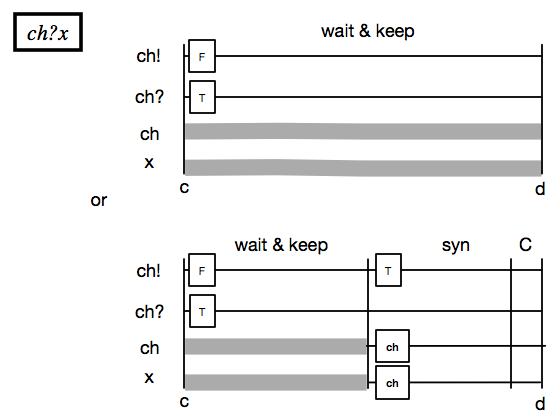
\includegraphics[width=0.9\columnwidth]{img/ChannelInput}}
  \caption{Graphical depiction of the HCSP channel input semantics}
  \label{fig:ChannelInput}
\end{figure}

Analogous to \ref{fig:ChannelOutput}, this diagram pair discusses the
two cases that satisfy the $ch?x$ term. In the top diagram, $ch!$ evaluates to
tt., while $ch?$ to ff.. In this case the values
of $ch$, and $x$ are irrelevant and the behaviour of the term is
simply $wait \wedge keep$.  In a equivalent manner in the bottom
diagram the interval is subdivided in three phases:
\begin{itemize}
\item In the first phase, $ch?$ is $false$, $ch!$ evaluates to $true$,
  so the behaviour is $wait \wedge keep$.
\item Once $ch?$ turns to $true$, we move to the $syn$ phase where
  value on ch is moved to x.
\item The last phase of the behaviour describes, again, the
  continuation sequence.
\end{itemize}

In POE/POE-$\Delta$, the ch?x HCSP term is represented with the
\mybox{ch?x} domain with the semantics: $\llbracket
ch?x \rrbracket \lceil \rceil$.

\paragraph{Value Assignment: y:=x}
The last primitive term, the assignment operation, which is visualised
in Figure \ref{fig:Assignment} simply sets the value of $y$ to the
values of $x$ in the time interval - $[c, d]$
\begin{figure}[hbt]
  \centering{
    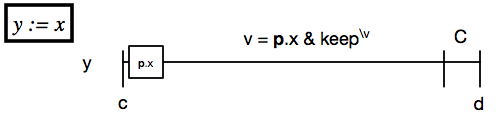
\includegraphics[width=0.9\columnwidth]{img/Assignment}}
  \caption{Graphical depiction of the Assignment semantics}
  \label{fig:Assignment}
\end{figure}

The POE/POE-$\Delta$ representation of the Value Assignment term is
\mybox{y := x} domain with the semantics: $\llbracket
y := x\rrbracket \lceil \rceil$.

\paragraph{Building complex terms from primitives}
For scaling up to real live systems, the HCSP primitive terms can be
combined into complex expressions using compositional operators like
sequential and parallel composition, as this is the case in our
example - $ch!5 || (ch?x; y := x)$.  First, let's look at the
sequential operator. In HCSP the sequential operator is defined as
follows:
\[\footnotesize\begin{array}{rcll}
                 \llbracket P; Q \rrbracket C \triangleq \llbracket P \rrbracket(\llbracket Q \rrbracket C)
               \end{array}\]

             The following Figure \ref{fig:Sequence} depicts the
             semantic of the sequence operator. The time interval
             $[c, d]$ is split into two subintervals: $[c, e]$ which
             is assigned to $P$ and $[e, d]$ which is assigned to $Q$,
             where $c < e < d$.  The satisfiability, and thus the
             result of the expression depends on the existence of a
             value $'v'$, for which the first HCSP term returns true
             in it's dedicated subinterval. If such a value exists the
             control flow is passed to the second term and its return
             value is then returned as the return value of the
             composite expression.

\begin{figure}[hbt]
  \centering{
    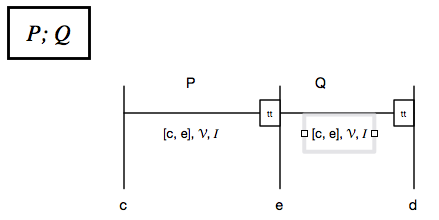
\includegraphics[width=0.9\columnwidth]{img/Sequence}}
  \caption{Graphical depiction of the sequential operator semantics}
  \label{fig:Sequence}
\end{figure}

The other operator used in the example is the parallel composition
operator, whose semantic is defined as follows:
\[\footnotesize\begin{array}{rcll}
                 \llbracket P || Q \rrbracket  \triangleq && \llbracket P \rrbracket skip \wedge \llbracket Q \rrbracket skip \\
                                                          && \vee \\
                                                          && \llbracket P \rrbracket skip \wedge \llbracket Q \rrbracket {stop}^{Q} \\
                                                          && \vee \\
                                                          && \llbracket P \rrbracket {stop}^{P} \wedge \llbracket Q \rrbracket skip
               \end{array}\]

             Figure \ref{fig:Parallel} visualises that semantic of the
             parallel operator, which given a time interval $[c, d]$
             gives control to both processes $P$, and $Q$.

\begin{figure}[hbt]
  \centering{
    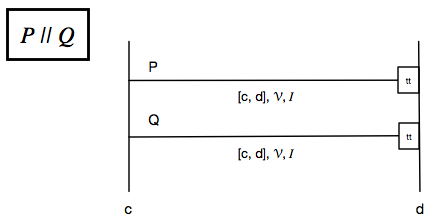
\includegraphics[width=0.9\columnwidth]{img/Parallel}}
  \caption{Graphical depiction of the sequential operator semantics}
  \label{fig:Parallel}
\end{figure}

The POE/POE-$\Delta$ representation of the sequencial and parallel
composition are the sequencial, respectively the parallel HCSP
domains: \mybox{ $\parallel$ }, \mybox{ ; }. 


\paragraph{Application of HCSP in POE/POE-$\Delta$}
As shown in the previous section we use the notion of HCSP unit
domains,to represent each HCSP primitive as a POE/POE-$\Delta$ unit
domain and plot it in a problem diagram. Additionally, we use the
POE/POE-$\Delta$ idea of shared phenomena, represented as arc
annotations to capture information about shared state as well to
coordinate the flow of execution.
Figure \ref{fig:ProblemHCSP} shows a problem diagram representing our
running example from the previous section.

\begin{figure}[hbt]
  \centering{
    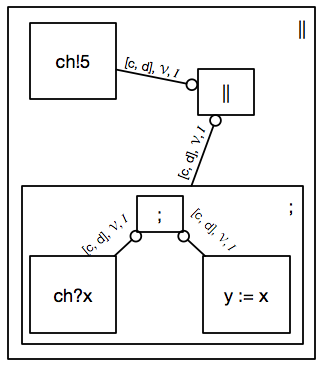
\includegraphics[width=0.9\columnwidth]{img/ProblemHCSP}}
  \caption{Graphical representation of the $ch!5 || (ch?x; y := x)$
    example in POE}
  \label{fig:Parallel}
\end{figure}

In the context of HCSP, the original POE/POE-$\Delta$ problem definition: \[E(S)\meets_{G}N\]
which reads ``Find $S$ which, when installed in $E$, meets $N$ to the
satisfaction of $G$.'' can be reinterpreted as:
\[
  \forall v \in \mathcal{V}, i \in \mathcal{I}ntv(E)
  \mathcal{L}([E](S)), v, i = tt.
\]
meaning that for all initial assignments $\mathcal{V}$, and for all
Intervals 'i' which are allowed for E, the interpretation of ([E](S))
in Interval 'i' and with valuation 'v' which evaluate to true satisfy
the need N.

In such a way we can use the higher level reasoning capabilities
offered by POE/POE-$\Delta$, while remaining fully compatible with the
precise and executable semantics of HCSP.
In the following we use the example of the Inventory Management
SystemS) from Chaochen's paper \citep{chaochen1996formal} to show how
it can be represented in POE/POE-$\Delta$ using the notion of HCSP
domain and how this can help us to reason about design.

%\todo{add IMS example}

\section{Conclusion}
\label{sect:Conclusion}
TBD

% ---------------------------------------------------------------------
% BIBLIOGRAPHY
% ---------------------------------------------------------------------
\frenchspacing \bibliographystyle{wileyauy} \bibliography{Literature}

\end{document}
